% !TEX root = ./amsa_main.tex
\section{Introduction}
This paper studies the \emph{coordinate update method}, which reduces a large problem to smaller subproblems and, thus, is useful for solving large-sized problems. This method handles both  linear and nonlinear maps, smooth and nonsmooth functions, and convex and nonconvex problems. Coordinate update algorithms generalize the coordinate descent algorithm  by relaxing the form of an update from coordinate-wise minimization to other forms. The most common examples of these algorithms are the Jacobian and Gauss-Seidel algorithms for solving linear equations. Coordinate update algorithms are also commonly found for solving differential equations (e.g., \emph{domain decomposition}) and optimization problems (e.g., \emph{coordinate descent}).  

After coordinate update algorithms are initially introduced in each topic area, their developments  slowed down until recently, when modern applications in signal and image processing, statistical and machine learning, and data-driven tasks  routinely involve a large amount of data; consequently,  numerical methods of \emph{small footprints} become increasingly popular. Since coordinate update algorithms decompose a large problem into much smaller subproblems, they tend to have low complexities and low memory requirements at each step. In addition, their implementations tend to be simpler and more amenable to taking advantages of existing numerical packages. 

The coordinate update method generates simple subproblems by fixing all but one variable, or a small block of variables. The updating variable can be selected in  the \textit{cyclic}, \textit{random}, or \textit{greedy} orders, making the method flexible and adaptive to specific problems. The form of subproblem varies depending on both the subproblem structure and the tradeoff between exactness and complexity. Different subproblems can be solved either sequentially in a single thread or concurrently in multiple threads, or even in an asynchronous parallel fashion. Therefore, coordinate update algorithms give rise to powerful numerical algorithms for large-scale problems.

\cut{\begin{table}
\begin{center}
\begin{tabular}{c|c|c}
\hline
Benefits & Coordinate Update & Full Update\\\hline\hline
memory footprint & small & big \\\hline
per iteration complexity & $O(n)$ & $O(n^2)$\\\hline
epoch & less (depend on updating order and stepsize) & more \\\hline
scalability & scalable & not scalable\\\hline
\end{tabular}
\end{center}
\caption{Benefits of coordinate update}\label{table:benefits}
\end{table}}

Regardless its update order, a coordinate update algorithm is \emph{computationally worthy} only if updating each coordinate, or each small block of coordinates, is much cheaper than updating all the coordinates together. When this assumption fails to hold, coordinate update is at a disadvantage to the full update (to all the coordinates). For example, given a $C^2$ function $f:\RR^n\to \RR$, consider the Newton update  $x^{k+1} \gets x^k - \big(\nabla^2 f(x^k)\big)^{-1}\nabla f(x^k)$. Since updating only a single $x_i$ (keeping other components fixed), in general, still requires forming $\nabla^2 f(x)$ (taking $O(n^2)$ operations) and factorizing it (taking $O(n^3)$ operations), there is little save in computation compared to updating all the components of $x$; hence, the Netwon's method is generally not amenable to coordinate update.  Therefore, identifying the favorable structures is the key to develop coordinate update algorithms.

The existing coordinate-update literature mostly focuses on introducing new algorithms, analyzing their convergence, and applying them to specific (classes of) problems with skillful improvements. \S\ref{sec:literature} below will review the literature. This paper, however, has a different focus:  the  components of  an efficient coordinate-update algorithm and their structures. We do not limit our discussion to specific update orders, update forms,  or classes of applications. We also largely ignore convergence guarantees \rev{(except that we provide convergence proof for a novel primal dual coordinate update method)} though they are important. Instead,   
%DIF > In this paper, we develop 
the developed coordinate update algorithms in this paper %DIF > for solving the In this paper, we try to find out when coordinate update algorithms can efficiently
solve the abstract fixed-point problem
\beq\label{fpprob}
x = \cT x,
\eeq
where  $\cT:\HH \to \HH$ is an operator and $\HH$ is a Hilbert space. 
 %GThe equation~\eqref{fpprob} encodes the solution to a lot of problems. 
For a  problem defined on $\HH$ and a given iterative algorithm for the problem,  we can let  $\cT$ abstract each iteration of the algorithm:
\beq\label{fpi}
x^{k+1} = \cT x^k.
\eeq
The limit of the sequence $\{x^k\}$  is a fixed point of $\cT$ and also a solution to the underlying problem. The update scheme~\eqref{fpi} generalizes iterative methods for solving linear equations, gradient descent, proximal gradient method,  operator splitting methods, and many other methods.

We study the structures of $\cT$ that make the  following coordinate update algorithm \emph{computationally worthy}
\beq\label{cuitr}
%x^{k+1}_i = (\cT x^k)_i\quad\mbox{or}\quad 
x^{k+1}_i = x_i^k - \eta_k (x^k-\cT x^k)_i,
\eeq
where $x_i$ is a coordinate of $x$ and $\eta_k$ is a  step size. We define the so-called \textbf{Coordinate Friendly (CF)} operator and provide examples. \cut{For $T=T_1+T_2$ or $T=T_1\circ T_2$, we discuss the structures of $T_1$ and $T_2$ that yield a CU friendly $T$.}

We construct coordinate update algorithms based on CF operators for a variety of problems including, but not limited to, linear programming, second-order cone programming, variational image processing, support vector machine, empirical risk minimization, portfolio optimization, and nonnegative matrix factorization. For each problem, we present an algorithm in the form of~\eqref{fpi} so that its coordinate update~\eqref{cuitr} is efficient. A final coordinate update algorithm can be obtained by plugging~\eqref{cuitr} into an algorithmic framework reviewed in \S\ref{sec:literature}. \rev{In this way we obtain new coordinate update algorithms for problems that were not treated with coordinate update before. For the problems with coordinate update solution, we recover the existing methods and also provide new approaches.}
\cut{\rev{We would like to point out our coordinate update scheme is different from the domain decomposition approach. Domain decomposition splits the variable domain into small subdomains and solves the original problem in each subdomains, with variables coherent on the intersections or the boundary. Our coordinate update scheme, on the other hand, is based on operator splitting. Variables are divided into coordinates corresponding to the algorithm instead of any physical grid domains and updating each coordinate involves solving a subproblem different from the original one. 
}
}

The algorithms developed in this paper are generalizations to many algorithms that are recently developed primarily for empirical risk minimization problems in machine learning. %and that solve so-called \emph{prox-linear} subproblems.
The generalization empowers us to solve more problems, such as those with multiple functions and constraints, as well as saddle-point formulations and variational inequalities.


In addition, the developed coordinate update algorithms can run on multiple agents in a parallel and even asynchronous fashion. This gives rise to parallel and asynchronous extensions to  existing algorithms including the Alternating Direction Method of Multipliers (ADMM), primal-dual splitting algorithms, and others.

The paper is organized as follows. \S\ref{sec:literature} reviews the existing frameworks of coordinate update algorithms. \S\ref{sec:cuf} discusses the underlying structures of CF operators. \S\ref{sec:comp-cuf} reviews operator splitting methods and presents composite CF operators. \S\ref{sec:p-d} reviews primal-dual splitting methods \rev{and introduces a new asynchronous primal dual coordinate update algorithm with convergence guarantee}. Based on the results of previous sections, \S\ref{sec:applications} introduces \rev{novel} coordinate update algorithms for various applications, some of which have been tested with numerical results presented in \S\ref{sec:numerical}.

Throughout this paper, all functions $f,g,h$ are proper closed convex and can take the extended value $\infty$, and all sets $X,Y,Z$ are nonempty closed convex. \cut{, and  an operator $\cT:\HH\to\HH$ is single-valued unless otherwise stated.} The indicator function $\iota_X(x)$ returns $0$ if $x\in X$, and $\infty$ elsewhere.


\cut{


decompose  the variables in a large problem into a number of small blocks, giving rise to simple subproblems that have low complexity, small memory footprints, and can be solved either sequentially or in parallel. 


Coordinate methods perform coordinate updates by keeping the other coordinates fixed. This often reduces to a lower dimensional subproblem and has lower per iteration computation complexity and space complexity compared to the fully update. This type of methods are often easy to implement.

For huge scale problems, there is a strong demand to solve the problem in a parallel, distributed and decentralized fashion. This is also in conformity with the ever increasing power of high performance computing systems.  However, due to the sequential (Gauss-Seidel approach) nature, it is often not straightforward to parallelize BC methods.]

We study the 

The goal of this paper is to identify CF maps where parallelization can be applied without incurring high overhead.}

\subsection{Coordinate Update Algorithmic Frameworks}\label{sec:literature}
This subsection reviews the  \emph{sequential} and \emph{parallel} algorithmic frameworks for coordinate updates, as well as the relevant literature. They give rise to coordinate update algorithms once their components such as $(\cT x^k)_i$ and $(x^k-\cT x^k)_{i}$ are realized for specific problems.

\subsubsection{Sequential Update} In this framework, there is a sequence of coordinate indices $i_1,i_2,\ldots$, and at each iteration $k=1,2,\ldots,$ only the $i_k$th coordinate is updated:
$$ \begin{cases}
x^{k+1}_{i} = x_{i}^k - \eta_k(x^k-\cT x^k)_{i},& i=i_k,\\
x^{k+1}_{i} = x_i^k,&\text{for all } i\not= i_k.
\end{cases}
$$
Sequential updates have been long known for special types of problems and their corresponding operators $\cT$, for example, the Gauss-Seidel iteration for solving linear equations, alternating projection \cite{von1949rings,bauschke1993convergence} for finding a point in the intersection of two sets,  ADMM \cite{glowinski1975ADMM, gabay1976ADMM} for solving monotropic programs, and Douglas-Rachford Splitting (DRS) \cite{douglas1956DRS}  for finding a zero to the sum of two operators. (ADMM and DRS also introduce and update additional variables.) 

In optimization,  \emph{coordinate descent} algorithms, at each iteration, minimize the function $f(x_1,\ldots,x_n)$ by fixing all but one variable. Let $$x_{-i}:=(x_1,\ldots,x_{i-1},x_{i+1},\ldots,x_n),$$
collect all but the $i$th coordinate of $x$. Coordinate descent updates take one of the following forms:
\begin{subequations}\label{coordes}
\begin{align}
(\cT x^k)_i & = \argmin_{x_i}f(x_i,x_{-i}^k),\\
(\cT x^k)_i & = \argmin_{x_i}f(x_i,x_{-i}^k)+\frac{1}{2\eta_k}\|x_i-x_i^k\|^2,\\
(\cT x^k)_i & = \argmin_{x_i}\,\langle \nabla_i f(x^k),x_i \rangle+\frac{1}{2\eta_k}\|x_i-x_i^k\|^2,\\
(\cT x^k)_i & = \argmin_{x_i}\,\langle \nabla_i f^{\mathrm{diff}}(x^k),x_i \rangle+f_i^{\mathrm{prox}}(x_i)+\frac{1}{2\eta_k}\|x_i-x_i^k\|^2,
\end{align}
\end{subequations}
which are called \emph{direct} update, \emph{proximal} update,  \emph{gradient} update, and \emph{prox-gradient} update, respectively. The last update applies to the function $$f(x) = f^{\mathrm{diff}}(x)+\sum_{i=1}^nf^{\mathrm{prox}}_i(x_i),$$ where $f^{\mathrm{diff}}$ is differentiable and each $f^{\mathrm{prox}}_i$ is proximable (its proximal map takes $O\big(\dim(x_i)\,\mathrm{polylog}(\dim(x_i))\big)$ operations).

%If the objective function has a \emph{proximable}+smooth structure,  the \emph{prox-gradient} update applies the proximal update to the result of the gradient update.  

\textbf{Sequential-update literature.} Coordinate descent algorithms date back to the 1950s~\cite{hildreth1957quadprog}, when the \emph{cyclic} update-order was used. Its convergence has been established under a variety of cases, for both convex and nonconvex objective functions; see~\cite{Warga-63,zadeh1970note, Sargent-Sebastian-73,Han-88,luo1992convergence, Tseng-93, Grippo-Sciandrone-00, Tseng-01, razaviyayn2013unified, beck2013convergence, hong2015iteration, wright2015coordinate}. Proximal updates are studied in~\cite{Grippo-Sciandrone-00, attouch2010proximal} and developed into prox-gradient updates in~\cite{tseng2009_CGD, tseng2009block-linear, bolte2014proximal} and mixed updates in~\cite{XY_2013_multiblock}.

The \emph{stochastic} update-order appeared in~\cite{nesterov2012cd} and then~\cite{richtarik2014iteration, Lu_Xiao_rbcd_2015}. Recently,~\cite{XY_2014_ecd,Xu2015_APG_NTD} compared the convergence speeds of cyclic and stochastic update-orders. The gradient update has been relaxed to  stochastic gradient update for large-scale problems in~\cite{DangLan-SBMD, XY_2015_bsg}. 

The \emph{greedy} update-order leads to fewer total iterations but is often impractical since it requires a lot of effort to calculate  scores for all the coordinates. However, there are cases where calculating the scores is easy~\cite{bertsekas1999nonlinear, li2009gcoord, wu2008coordinate} and the save in the total iterations significantly outweighs the effort \cite{tseng2009_CGD, dhillon2011nearest, PYY_2013_GRock, schmidt2014coordinate}. 

\textbf{A simple test.} Although our purpose is not to compare different update-orders, we feel necessary to make them concrete for the reader. For simplicity, we adopt the least squares problem
$$\Min_{x} \frac{1}{2} \|A x - b\|^2,$$
where $A \in \RR^{p \times m}$ and $b \in \RR^p$ are Gaussian random, to numerically demonstrate the advantages of coordinate updates over the  full update of  gradient descent:
$$x^{k+1} = x^k - \eta_k A^{\top}(A x^k - b).$$
The four coordinate update schemes are: cyclic, cyclic permutation, random, and greedy under the Gauss-Southwell rule. 
In the full update, the step size $\eta_k$ is set to the theoretical upper bound $\frac{2}{\|A\|_2^2}$. For each coordinate update to $x_i$, the step size $\eta_k$ is set to $\frac{1}{(A^{\top}A)_{ii}}$. All of the full and coordinate updates have the same \emph{per-epoch} complexity, so we plot the objective errors in Figure \ref{fig:ls_full_vs_coord}. 
Note that the performance of coordinate update algorithms depend on many factors such as the condition number, the level of coupling among different coordinates, whether greedy selections can be efficiently made, as well as the amount of data move needed. The demonstration here is limited. 
\begin{figure}[!htbp] \centering
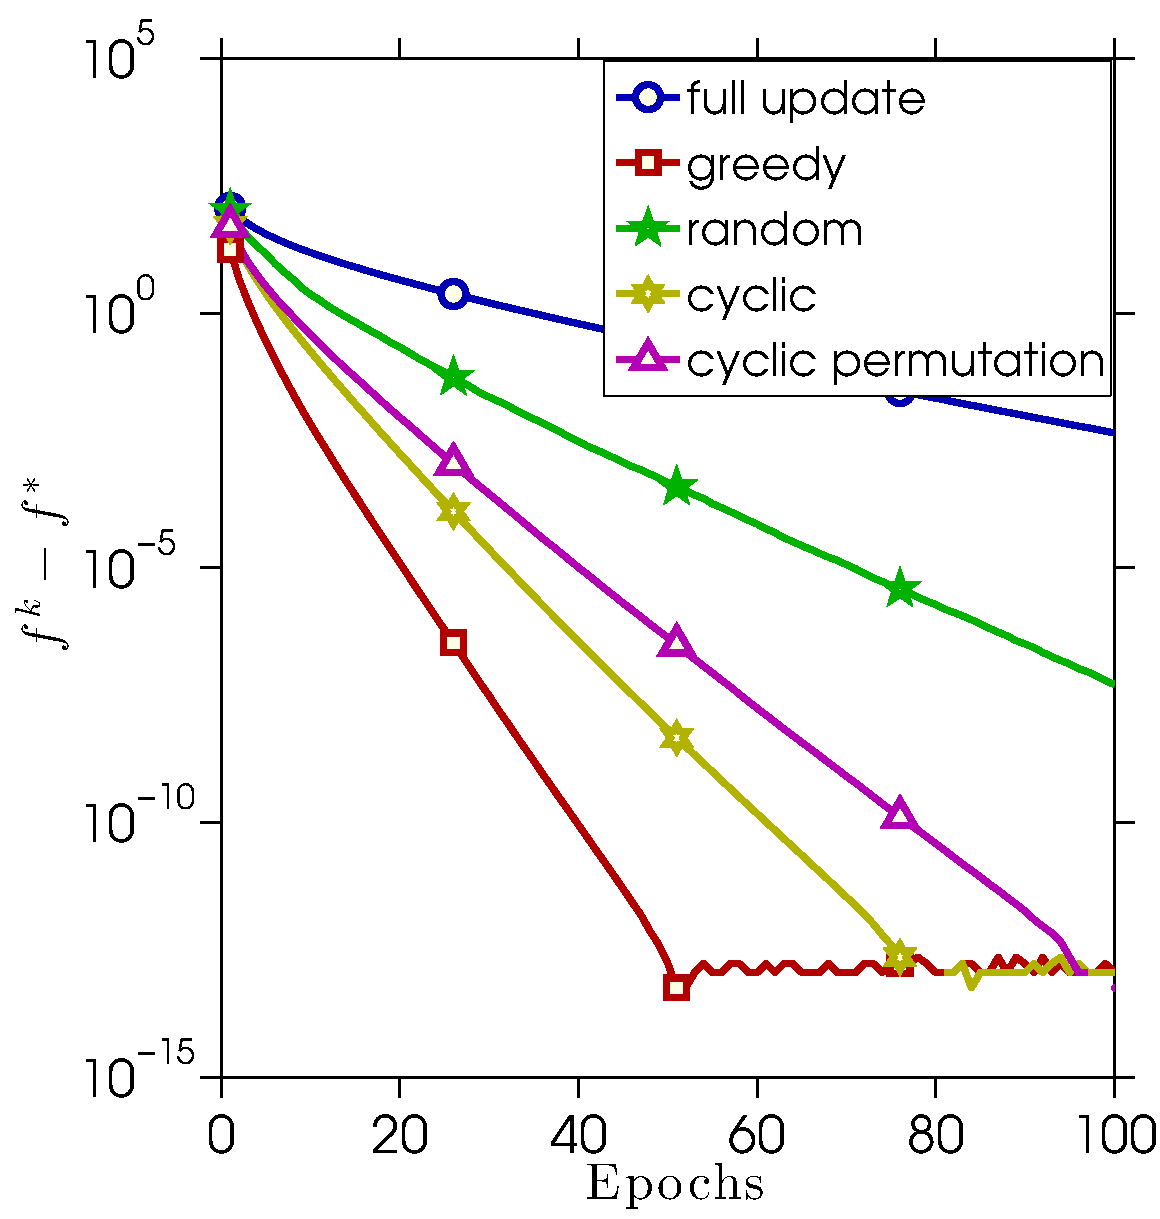
\includegraphics[width=50mm]{./figs/randn_matrix_cropped}

\caption{Gradient descent: the coordinate updates are faster than the full update since the former can take larger steps at each step.}
\label{fig:ls_full_vs_coord}
\end{figure}



\subsubsection{Parallel Update} We discuss both synchronous (sync) and asynchronous (async) versions of parallel updates.

\textbf{Sync-parallel (Jacobi) update.} In this framework, there is a sequence of index sets $\II_1,\II_2,\ldots$ (which are subsets of $\{1,\ldots,n\}$), and at each iteration $k=1,2,\ldots,$  the coordinates in $\II_k$ are updated in parallel by multiple agents:
$$ \begin{cases}
x^{k+1}_{i} = x_{i}^k - \eta_k(x^k-\cT x^k)_{i},& i\in \II_k,\\
x^{k+1}_{i} = x_i^k,&i\not\in \II_k.
\end{cases}
$$
The counter $k$ increases after all coordinate updates in $\II_k$ are completed. If $\II_k=\{1,\ldots,n\}$, then all the coordinates are updated; hence, each iteration reduces to the standard update: $x^{k+1} =  x^k - \eta_k(x^k-\cT x^k).$ \cut{\color{red}This, of course, does not mean solving $x=\cT x$ in one step; therefore, do not confuse performing an  update in \eqref{coordes} for all the coordinates in parallel from the joint minimization over all the variables.}

\textbf{Async-parallel update.} In this framework, a set of agents  perform simultaneous updates that  are aligned up in time. Each of them continuously applies \eqref{fm:async} below to the variable   $x$  in the shared memory (or locally storing $x$ and communicating with other agents):  
\beq\label{fm:async} \begin{cases}
x^{k+1}_{i} = x_{i}^k - \eta_k \left((\cI-\cT) x^{k-d_k}\right)_{i},& i=i_k,\\
x^{k+1}_{i} = x_i^k,& \text{for all }i\not= i_k.
\end{cases}
\eeq
Here, $k$ increases  whenever one agent completes an update, and $d_k$ is the asynchronous delay. 

\begin{figure} \centering
    \begin{subfigure}[b]{0.45\linewidth}
        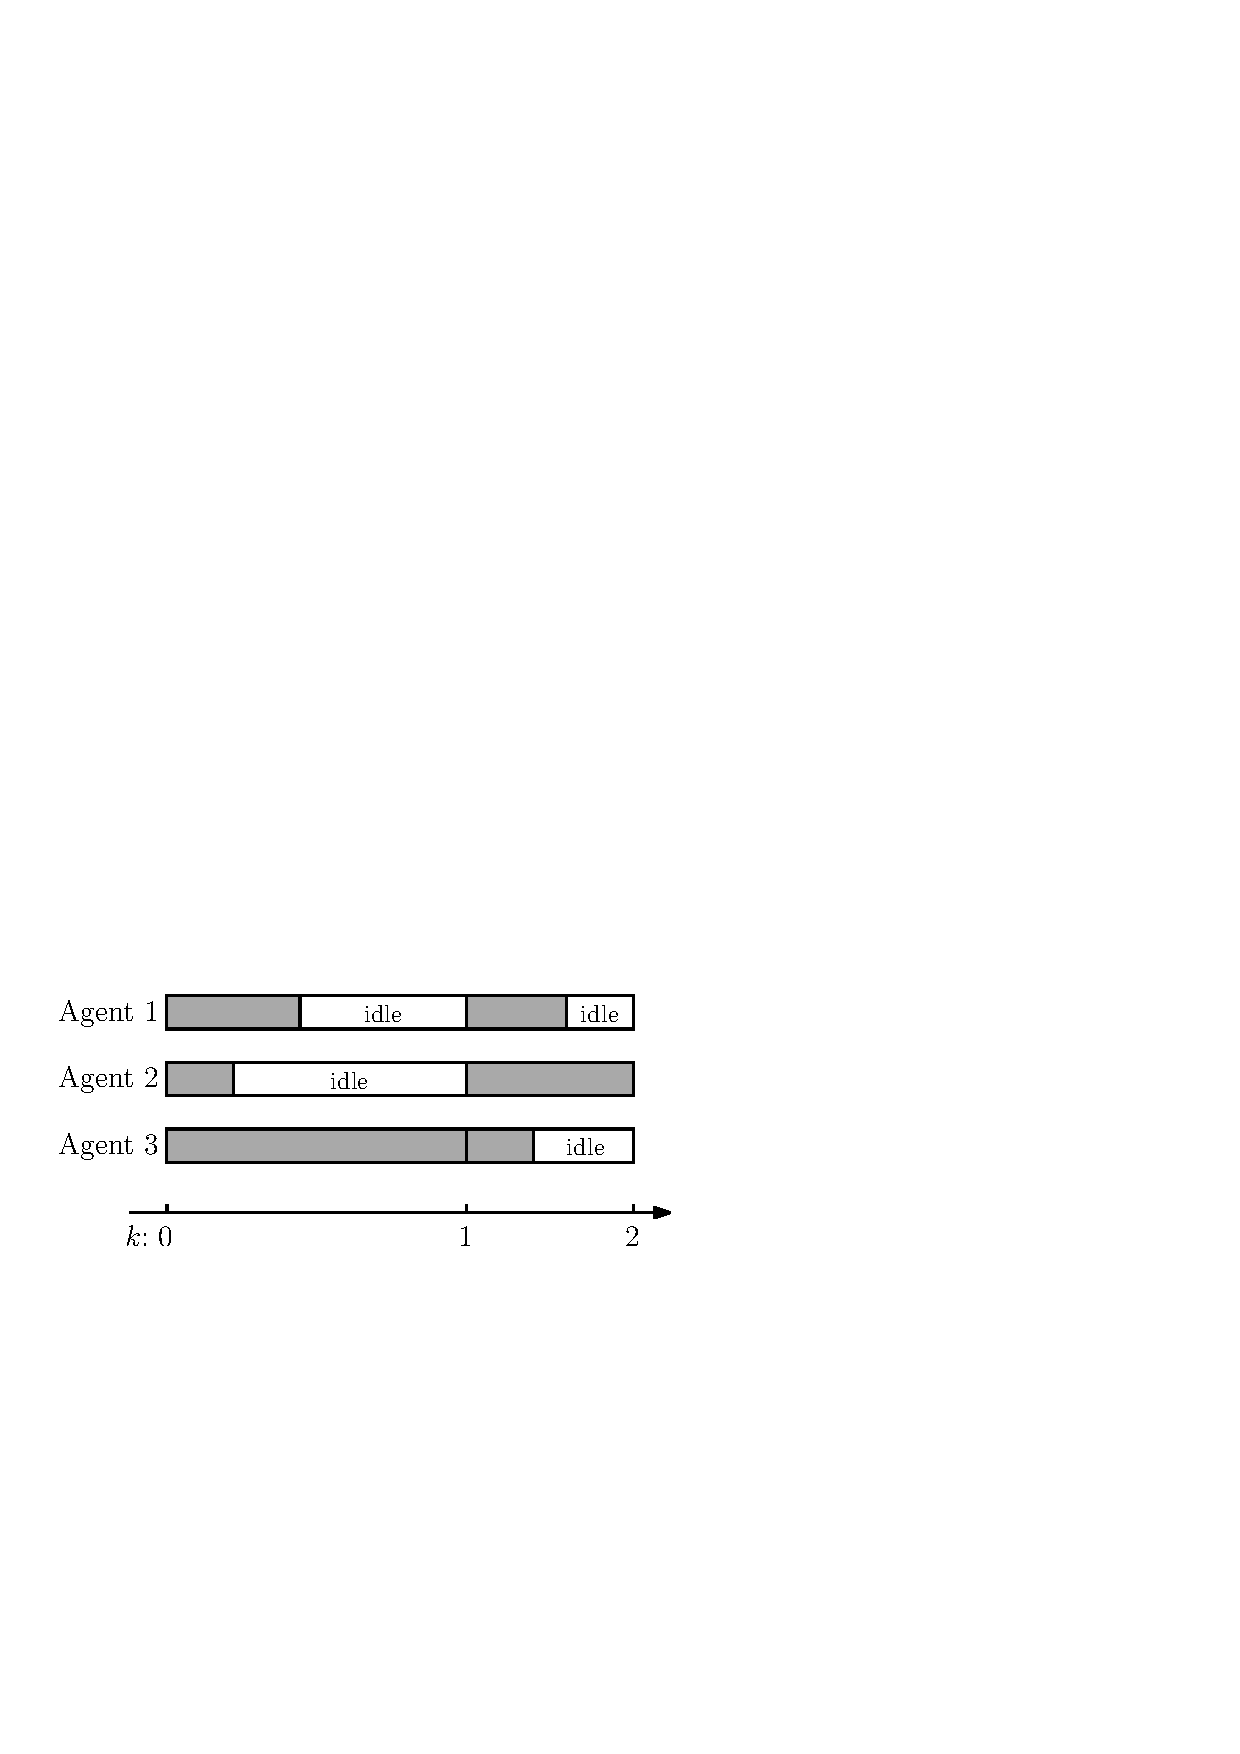
\includegraphics[width=60mm]{./figs/syn-simple}
        \caption{sync-parallel computing}
        \label{fig:parallel_a}
    \end{subfigure} %
    \quad
    \begin{subfigure}[b]{0.45\linewidth}
        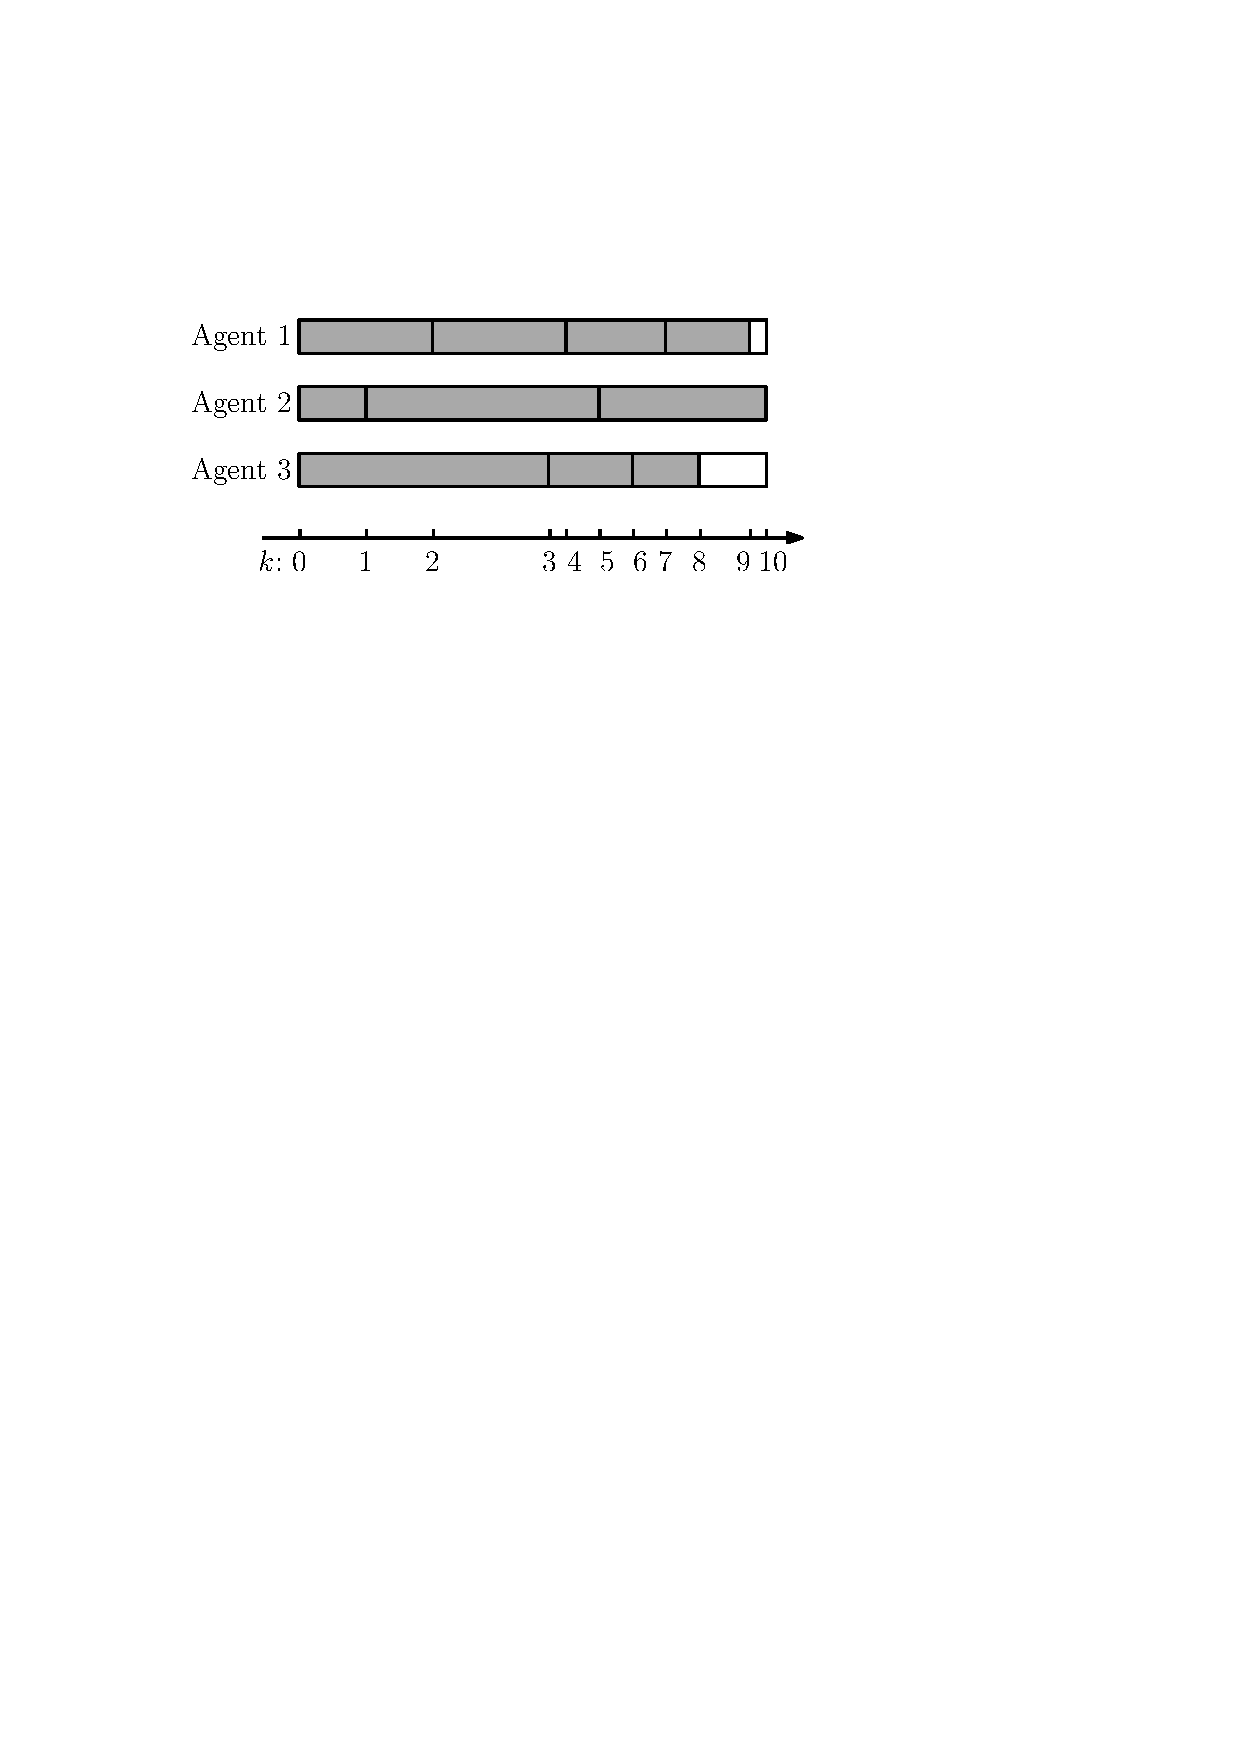
\includegraphics[width=60mm]{./figs/asyn-simple}
        \caption{async-parallel computing}
        \label{fig:parallel_b}
    \end{subfigure} %
    \caption{ Sync-parallel computing (left) versus async-parallel computing (right). On the left, all the agents must wait at idle (white boxes) until the slowest agent has finished.}
    \label{fig:comp_sync_async}
\end{figure}

% \begin{center}[picture: sync-parallel vs async-parallel]\end{center}

At each sync-parallel iteration, synchronization must wait for the completion of the last (slowest) update. %It is not truly scalable since, as the number of agents increase, the slowest update  becomes slower and also because it is not fault tolerant. In addition, in the synchronous algorithm, all the processors simultaneously make congestion-inducing communication and memory-access requests.
Async-parallel updates eliminate such idle time, spread out memory access and  communication, and is generally  more fault-tolerant. However, async-parallel is less stable and more difficult to analyze because of the asynchronous delay.

Asynchronous delay occurs if, after an agent reads $x$ yet before it completes updating $x_{i_k}$, other agents also make updates to $x$. In~\eqref{fm:async}, the agent reads $x^{k-d_k}$ and commits the update to $x_{i_k}^k$. The delay $d_k$ equals the number of updates by other agents during this period. Here we assume the \emph{consistent} case, i.e., $x$ read by one agent is in the history of $\{x^k\}$. For the \emph{inconsistent} case, please see~\cite[Section 1.2]{Peng_2015_AROCK} for more details.

%Here, $d_k$ is a scalar in the \emph{consistent} case and a vector in the \emph{atomically inconsistent} case. In the former case, the delays of the entries of $x^{k-d_k}$ are consistent, namely,  $x^{k-d_k}=[x^{k-d_k}_1,\ldots,x^{k-d_k}_n]$. \emph{Atomic inconsistency}, on the other hand, allows inconsistent delays: $x^{k-d_k}=[x^{k-d_{k,1}}_1,\ldots,x^{k-d_{k,n}}_n]$, where $d_k\in\NN^n$ is a vector and $n$ is the number of block coordinates. Inconsistency occurs when multiple agents read and write the entries of $x$ simultaneously, but  atomicity of $x_i$ ensures that all the sub-entries or bits of  $x_i$ are read and written at once and thus stay consistent.

\remove{The sync-parallel update is a special case of the async-parallel update where the number of agents equals $|\II_k|$ and  the asynchronous delay is uniformly zero.}

\textbf{Parallel-update literature.} 
Async-parallel methods can be traced back to~\cite{chazan1969chaotic} for linear systems. For function minimization,~\cite{bertsekas1989parallel} introduced an async-parallel gradient-projection method. Convergence rates are obtained in~\cite{tseng1991rate-asyn}.  
Recently, \cite{bradley2011parallel,richtarik2012parallel} developed parallel randomized methods. 

For fixed-point problems, async-parallel methods date back to~\cite{Baudet_1978_asynchronous} in 1978. In  the pre-2010 methods \cite{BMR1997asyn-multisplit,bertsekas1983distributed,Baz200591,el1998flexible} and the review~\cite{Frommer2000201}, each agent updates its own subset of coordinates. Convergence is established under the \emph{$P$-contraction} condition and its variants~\cite{bertsekas1983distributed}. Papers~\cite{Baz200591,Baz1998429} show convergence for async-parallel iterations with simultaneous reading and writing to the same set of components. Unbounded but stochastic delays are considered in~\cite{Strikwerda2002125}.

Recently, random coordinate selection appeared in~\cite{Patrick_2015} for fixed-point problems. The works \cite{nedic2001distributed,recht2011hogwild,liu2013asynchronous,liu2014asynchronous,hsieh2015passcode} introduced async-parallel stochastic methods for function minimization.
For fixed-point problems,~\cite{Peng_2015_AROCK} introduced  async-parallel stochastic methods, as well as several applications.  

\subsubsection{Contributions of this paper} 
The paper systematically discusses the CF structures found in both single and composite operators underlying many interesting applications. We introduce approaches to recognize CF operators and develop coordinate-update algorithms based on them. 
We provide a variety of applications to illustrate our approaches. 
In particular, we obtain new coordinate-update algorithms for image deblurring, portfolio optimization, second order cone programming, as well as tensor decomposition. Our analysis also provides guidance to the implementation of coordinate-update algorithms by specifying how to compute certain operators and maintain certain quantities in memory. \rev{We also provide numerical results to illustrate the efficiency of the proposed coordinate update algorithms.}
 
This paper does \emph{not} focus on the convergence perspective of coordinate update algorithms (or coordinate descent for function minimization), \rev{except that we provide the convergence proof of our async-parallel primal-dual coordinate update algorithm in the appendix}. In general, in fixed-point algorithms, the iterate convergence is ensured by the monotonic decrease of the distance between the iterates and the solution set, while in minimization problems, the objective value convergence is ensured by the monotonic decrease of a certain energy function. The reader is referred to the existing literature for details. 

%{\color{red}In general, their convergence are ensured by a certain monotonically decreasing energy function in unconstrained minimization, giving  objective value convergence, and by the  monotonically decreasing distance to the solution set in fixed-point problems, giving point convergence (and objective value convergence if applied to minimization). }

In our fixed-point setting, the operator $\cT$ generally needs to be  nonexpansive (under a certain metric). The operator splitting methods reviewed in~\S\ref{sec:comp-cuf} below generate nonexpansive operators $\cT$ for many problems considered in this paper. The convergence of the resulting stochastic sequential and  (async)-parallel coordinate-update algorithms, as well as their step size selections, is referred to the recent works~\cite{Patrick_2015,Peng_2015_AROCK}. On the other hand, the structure properties of operators discussed in this paper are irrelevant to nonexpansiveness or convexity. Hence, the algorithms developed can be still applied to nonconvex problems without guarantees.


%\end{subsection}

%\end{section}
% at solving large-sized problems involving  linear and nonlinear maps, and smooth and nonsmooth functions.  at solving large-sized problems involving  linear and nonlinear maps, and smooth and nonsmooth functions. 
 %DIF < \DIFdelbegin \DIFdel{It handles both  linear and nonlinear maps, and smooth and nonsmooth functions. The most common examples  }\DIFdelend %DIF > It handles both  linear and nonlinear maps, and smooth and nonsmooth functions. The most common examples 
